\documentclass{beamer}
\usepackage{algorithm} %pseudo-code
\usepackage{algpseudocode}
\usepackage{amsmath, amssymb, amscd}
\usepackage{graphicx}
\usepackage{float}
\usepackage{amsmath, amssymb, amscd}
\usepackage{alltt}
\usepackage{textcomp}
\usepackage{gensymb}
\usepackage{multicol}
\usepackage{tabularx}

\newcommand{\N}{\mathbb{N}}
\newcommand{\Z}{\mathbb{Z}}
\newcommand{\R}{\mathbb{R}}
\newcommand{\bigo}{\mathcal{O}}
\newcommand{\G}{\mathcal{G}}
\newcommand{\V}{\mathcal{V}}
\newcommand{\E}{\mathcal{E}}
\newcommand{\K}{\mathcal{K}}
\newcommand{\T}{^\intercal}

\newcommand{\sups}[1]{\ensuremath{^{\textrm{#1}}}}
\newcommand{\subs}[1]{\ensuremath{_{\textrm{#1}}}}

\newcommand{\specialcell}[2][c]
{
  \begin{tabular}[#1]{@{}c@{}}#2\end{tabular}
}

\makeatletter
\newsavebox{\mybox}\newsavebox{\mysim}
\newcommand{\distras}[1]
{
  \savebox{\mybox}{\hbox{\kern3pt$\scriptstyle#1$\kern3pt}}%
  \savebox{\mysim}{\hbox{$\sim$}}%
  \mathbin{\overset{#1}{\kern\z@\resizebox{\wd\mybox}{\ht\mysim}{$\sim$}}}%
}
\makeatother
%===============================================================================
% code highlighting :
\usepackage{listings}

% define custom colors :
\usepackage{color}
\definecolor{bg}{rgb}{0.96,0.96,0.85}
\definecolor{deepblue}{rgb}{0,0,0.5}
\definecolor{deepred}{rgb}{0.6,0,0}
\definecolor{deepgreen}{rgb}{0,0.5,0}

\usepackage{xcolor}
\renewcommand{\lstlistlistingname}{Code Listings}
\renewcommand{\lstlistingname}{Code Listing}
\definecolor{gray}{gray}{0.5}
\colorlet{commentcolour}{green!50!black}

\colorlet{stringcolour}{red!60!black}
\colorlet{keywordcolour}{magenta!90!black}
\colorlet{exceptioncolour}{yellow!50!red}
\colorlet{commandcolour}{blue!60!black}
\colorlet{numpycolour}{blue!60!green}
\colorlet{literatecolour}{magenta!90!black}
\colorlet{promptcolour}{green!50!black}
\colorlet{specmethodcolour}{violet}
\colorlet{indendifiercolour}{green!70!white}

\newcommand{\framemargin}{5ex}

\newcommand{\literatecolour}{\textcolor{literatecolour}}

\newcommand\pythonstyle{\lstset{
%keepspaces=true,
language=python,
showtabs=true,
tab=,
tabsize=2,
basicstyle=\ttfamily\scriptsize,%\setstretch{.5},
stringstyle=\color{stringcolour},
showstringspaces=false,
alsoletter={1234567890},
otherkeywords={\ , \}, \{, \%, \&, \|},
keywordstyle=\color{keywordcolour}\bfseries,
emph={and,break,class,continue,def,yield,del,elif ,else,%
except,exec,finally,for,from,global,if,import,in,%
lambda,not,or,pass,print,raise,return,try,while,assert},
emphstyle=\color{blue}\bfseries,
emph={[2]True, False, None},
emphstyle=[2]\color{keywordcolour},
emph={[3]object,type,isinstance,copy,deepcopy,zip,enumerate,reversed,list,len,dict,tuple,xrange,append,execfile,real,imag,reduce,str,repr},
emphstyle=[3]\color{commandcolour},
emph={Exception,NameError,IndexError,SyntaxError,TypeError,ValueError,OverflowError,ZeroDivisionError},
emphstyle=\color{exceptioncolour}\bfseries,
%upquote=true,
morestring=[s]{"""}{"""},
morestring=[s]{'''}{'''},
commentstyle=\color{commentcolour}\slshape,
%emph={[4]1, 2, 3, 4, 5, 6, 7, 8, 9, 0},
emph={[4]ode, fsolve, sqrt, exp, sin, cos, arccos, pi,  array, norm, solve, dot, arange, , isscalar, max, sum, flatten, shape, reshape, find, any, all, abs, linspace, legend, quad, polyval,polyfit, hstack, concatenate,vstack,column_stack,empty,zeros,ones,rand,vander,grid,pcolor,eig,eigs,eigvals,svd,qr,tan,det,logspace,roll,min,mean,cumsum,cumprod,diff,vectorize,lstsq,cla,eye,xlabel,ylabel,squeeze,plot,median,std,hist},
emphstyle=[4]\color{numpycolour},
emph={[5]__init__,__add__,__mul__,__div__,__sub__,__call__,__getitem__,__setitem__,__eq__,__ne__,__nonzero__,__rmul__,__radd__,__repr__,__str__,__get__,__truediv__,__pow__,__name__,__future__,__all__},
emphstyle=[5]\color{specmethodcolour},
emph={[6]assert,range,yield},
emphstyle=[6]\color{keywordcolour}\bfseries,
% emph={[7]self},
% emphstyle=[7]\bfseries,
literate=*%
{:}{{\literatecolour:}}{1}%
{=}{{\literatecolour=}}{1}%
{-}{{\literatecolour-}}{1}%
{+}{{\literatecolour+}}{1}%
{*}{{\literatecolour*}}{1}%
{/}{{\literatecolour/}}{1}%
{!}{{\literatecolour!}}{1}%
%{(}{{\literatecolour(}}{1}%
%{)}{{\literatecolour)}}{1}%
{[}{{\literatecolour[}}{1}%
{]}{{\literatecolour]}}{1}%
{<}{{\literatecolour<}}{1}%
{>}{{\literatecolour>}}{1}%
{>>>}{{\textcolor{promptcolour}{>>>}}}{1}%
,%
breaklines=true,
breakatwhitespace= true,
%xleftmargin=\framemargin,
%xrightmargin=\framemargin,
aboveskip=1ex,
frame=trbl,
%frameround=tttt,
rulecolor=\color{black!40},
%framexleftmargin=\framemargin,
%framextopmargin=.1ex,
%framexbottommargin=.1ex,
%framexrightmargin=\framemargin,
%framexleftmargin=1mm, framextopmargin=1mm, frame=shadowbox, rulesepcolor=\color{blue},#1
%frame=tb,
backgroundcolor=\color{yellow!10}
}}

% Python environment
\lstnewenvironment{python}[1][]
{
  \pythonstyle
  \lstset{#1}
}
{}

% Python for external files
\newcommand\pythonexternal[1]
{{
  \pythonstyle
  \lstinputlisting{#1}
}}

% Python for inline
\newcommand\pythoninline[1]{{\pythonstyle\lstinline!#1!}}

% end code highlighting
%===============================================================================


\begin{document}
\small

\title{Killer Yeast Vs. Sensitive Yeast}
\author{Evan Cummings \and Intizor Aliyorov \and Malachi J.\ Cryder\\
MATH 445 - Statistical, Dynamical, and Computational Modeling}

\maketitle

\section*{Proposal}
The differential equation we may use for modeling the growth of yeast is the same as that used for bacterial growth in a chemostat:
\begin{align*}
  \frac{dN}{dt} &= k(C) N - \frac{FN}{V}, \\
  \frac{dC}{dt} &= -\alpha k(C) N - \frac{FC}{V} + \frac{FC_0}{V},
\end{align*}
with initial conditions $C(0) = C_i$ and $N(0) = N_i$, $N$ is the unitless optical density of yeast in the chamber, $C$ is the unitless optical density of nutrient in the chamber, $C_0$ is the unitless optical density of nutrient in the reservoir, $F$ is the in/out volume flow rate with units volume/time, $V$ is the volume of the chamber, $\alpha$ is a unitless inverse of the yield constant, and $k(C)$ is the reproduction rate for yeast in units 1/time with possible formula chosen such that $\lim_{C \rightarrow \infty} = k_{max}$, and $k_{max}$ represents the maximum possible reproduction rate:
$$k(C) = \frac{k_{max} C}{C_n + C}.$$
where $C_n$ is chosen such that $k(C_n) = k_{max} / 2$.  Because the concentration in the tank $C(t)$ is related to the concentration in the reservoir by $C(t) \leq C_0$, $C_0$ may be chosen sufficiently small such that 
\begin{align*}
  k(C) = \frac{k_{max} C}{C_n + C} \approx \frac{k_{max} C}{C_n} = KC,
\end{align*}
where $K$ has units 1/time. The equations we need to solve then become 
\begin{align}
  \frac{dN}{dt} &= KCN - \frac{FN}{V}, \\
  \frac{dC}{dt} &= -\alpha KCN - \frac{FC}{V} + \frac{FC_0}{V}.
\end{align}
The quantitative measurement for fitness is a unitless measurement of optical density at steady state ($N$) at a given flow rate ($F$) in volumes/hr.  In order to find the steady states, we have to find the intersections of the null-clines at equilibrium points $(\bar{N}, \bar{C})$, i.e.\ $dN(\bar{N},\bar{C})/dt = 0$ and $dC(\bar{N},\bar{C})/dt = 0$:
\begin{align*}
  \frac{dN(\bar{N}, \bar{C})}{dt} &= K\bar{C} \bar{N} - \frac{F\bar{N}}{V}, \\
  &= \bar{N} \left( K\bar{C} - \frac{F}{V} \right) = 0, \\
\end{align*}
which is zero for $\bar{N} = 0$ or $K \bar{C} = F/V$.  Solving the other equation gives us the other steady-states:
\begin{align*}
  \frac{dC(\bar{N}, \bar{C})}{dt} &= -\alpha K \bar{C} \bar{N} - \frac{F\bar{C}}{V} + \frac{FC_0}{V} = 0,
\end{align*}
which is zero for $\alpha K\bar{C} \bar{N} + \frac{F\bar{C}}{V} = \frac{FC_0}{V}$.

In order to evaluate these null-clines, we need to evaluate the non-trivial cases, here for $\dot{N} = 0$,
\begin{align}
  K \bar{C} &= \frac{F}{V} \notag \\
  \implies \bar{C} &= \frac{F}{VK}.
\end{align}
Likewise, for $\dot{C} = 0$,
\begin{align}
  \alpha K \bar{C} \bar{N} + \frac{F\bar{C}}{V} &= \frac{FC_0}{V} \notag \\
  \implies \bar{N} &= \frac{FC_0}{V \alpha K \bar{C}} - \frac{F}{V \alpha K} = \frac{F}{V \alpha K} \left(\frac{C_0}{\bar{C}} - 1 \right).
\end{align}
This intersects the $\bar{N} = 0$ nullcline at $\frac{F}{V\alpha K} = 0$ or $\frac{C_0}{\bar{C}} = 1$.  However, because $F$ is never 0, we can disregard the first equation, and we know that the only trivial steady-state is located at $\bar{N} = 0$, $\bar{C} = C_0$.

\begin{multicols}{2}
\begin{figure}[H]
  \centering
    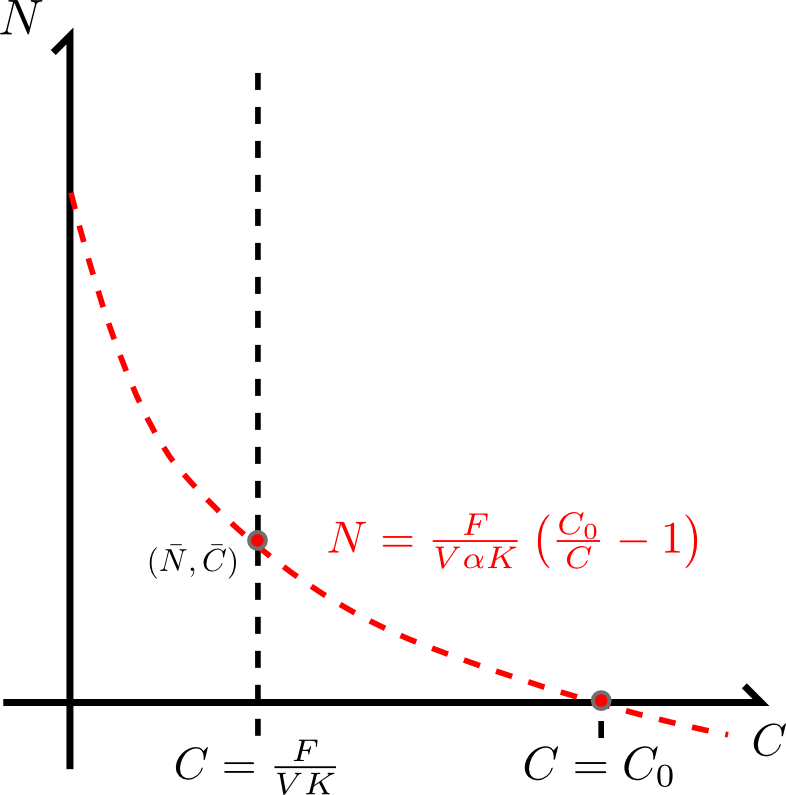
\includegraphics[width=0.35\textwidth]{images/drawing.png}
  \caption{\footnotesize The $\dot{C} = 0$ nullcline (dashed red) intersecting with the $\dot{N} = 0$ nullcline (dashed black).  The trivial and non-trivial steady-states $(0, C_0)$ and $(\bar{N}, \bar{C})$ are shown as red dots.}
\end{figure}
\vfill
\columnbreak
By placing Eq.\ (3) inside Eq.\ (4), we can find the non-trivial steady-state, the intersection of null-clines:
\begin{align}
  \bar{N}(\bar{C}) &= \frac{FC_0}{V \alpha K \bar{C}} - \frac{F}{V \alpha K}  \notag \\
  &= \frac{FC_0}{V \alpha K \frac{F}{VK}} - \frac{F}{V \alpha K} \notag \\
  &= \frac{C_0}{\alpha} - \frac{F}{V \alpha K} = \frac{1}{\alpha} \left( C_0 - \frac{F}{VK} \right).
\end{align}
The unknown parameters in Eq (5) are $\alpha$ and $K$.  We can find these parameters by fitting Eq (5) to the data by non-linear least squares fitting $\bar{N}_i$ at $F_i$ for $i = 1,\ldots,n$, where $n$ is the number of observations.
\end{multicols}

After we obtain estimates of these parameters for both the killer yeast $L$ and sensitive yeast $S$, ($\alpha_L$, $\alpha_S$ and $K_L$, $K_S$ respectively), we can model a ``what if'' scenario whereby we place both species of yeast, sensitive and killer, into one chemostat.  The population of sensitive yeast $S$ will be negatively impacted by the amount of toxin the killer yeast $K$ can produce, so we add the term $-\beta K L$ to the differential equation describing population $S$.  The differential equations we use to solve this three-species model is
\begin{align}
  \frac{dL}{dt} &= K_L CL - \frac{FL}{V}, \\
  \frac{dS}{dt} &= K_S CS - \frac{FS}{V} - \beta S L, \\
  \frac{dC}{dt} &= -\alpha_L K_L CL -\alpha_S K_S CS - \frac{FC}{V} + \frac{FC_0}{V}.
\end{align}


The data we are provided with include two sets of two separate runs, along with the concentration of nutrient in the reservoir, $C_0 = 0.02$:
\section{K1 Run}
\subsection*{Vessel One :}
\begin{tabular}{l|cccccccc}
  Volumes/Hr & 0.028 & 0.099 & 0.142 & 0.207 & 0.269 & 0.287 & 0.352 & 0.403 \\
  Optical Density at Steady State & 0.144 & 0.151 & 0.099 & 0.069 & 0.045 & 0.02 & 0.003 & 0 \\
\end{tabular}

\subsection*{Vessel Two :}
\begin{tabular}{l|ccccccccc}
  Volumes/Hr & 0.054 & 0.11 & 0.141 & 0.199 & 0.257 & 0.296 & 0.348 & 0.397 & 0.41 \\
  Optical Density at Steady State & 0.164 & 0.151 & 0.11 & 0.092 & 0.072 & 0.023 & 0.006 & 0.002 & 0.004 \\
\end{tabular}

\section{Sensitive Run}
\subsection*{Vessel One :}
\begin{tabular}{l|ccccccccc}
  Volumes/Hr & 0.041 & 0.099 & 0.167 & 0.223 & 0.266 & 0.328 & 0.356 & 0.401 & 0.462 \\
 Optical Density at Steady State & 0.54 & 0.494 & 0.459 & 0.395 & 0.229 & 0.019 & 0.006 & 0.003 & 0  \\
\end{tabular}

\subsection*{Vessel Two :}
\begin{tabular}{l|ccccccc}
 Volumes/Hr & 0.0571 & 0.126 & 0.196 & 0.263 & 0.313 & 0.383  \\
  Optical Density at Steady State & 0.385 & 0.456 & 0.363 & 0.197 & 0.044 & 0.004 \\
\end{tabular}

\begin{figure}[H]
  \centering
    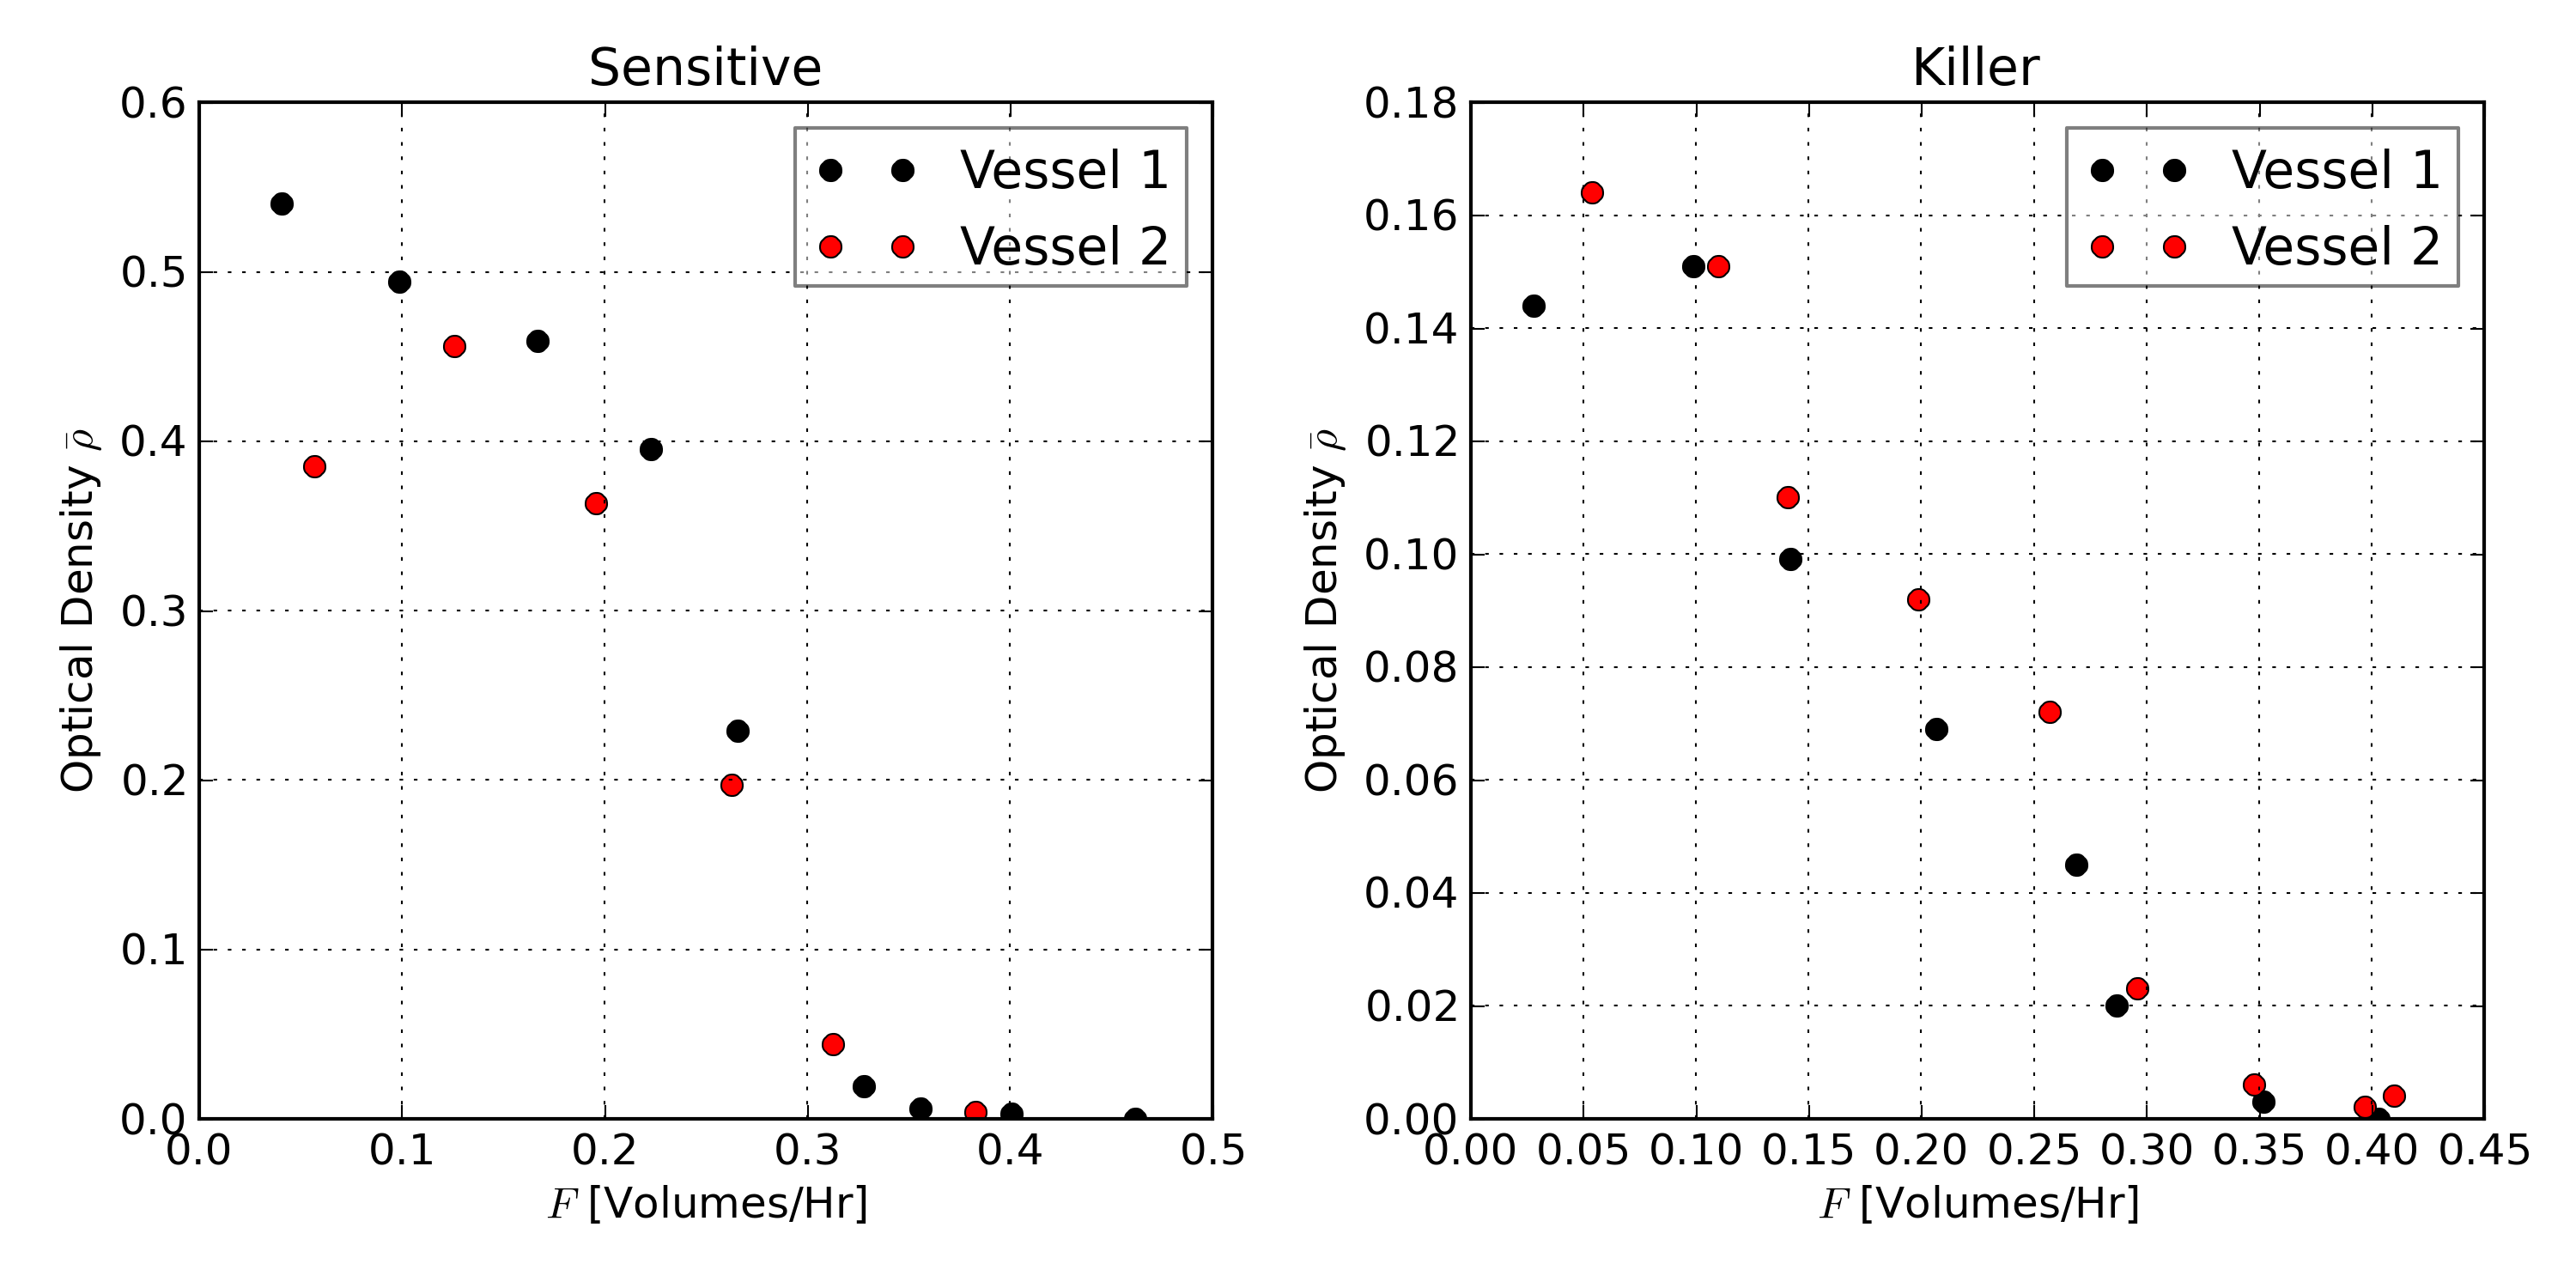
\includegraphics[width=1.0\textwidth]{images/data.png}
\end{figure}

The data provided does not include the volume of the chamber, $V$.  In order to solve Eq.\ (5), this quantity is needed.  Here we have dimensional analysis of the problem:

\begin{align*}
  \frac{dN}{dt} &= KCN - \frac{FN}{V} \\
  \equiv \left[ \frac{1}{\text{time}} \right] &\equiv \left[ \frac{1}{\text{time}} - \frac{\text{volume}}{\text{time}} \cdot \frac{1}{\text{volume}} \right] \equiv \left[ \frac{1}{\text{time}} \right], \\
  \frac{dC}{dt} &= -\alpha KCN - \frac{FC}{V} + \frac{FC_0}{V} \\
  \equiv \left[ \frac{1}{\text{time}} \right] &\equiv \left[ -\frac{1}{\text{time}} - \frac{\text{volume}}{\text{time}} \cdot \frac{1}{\text{volume}} + \frac{\text{volume}}{\text{time}} \cdot \frac{1}{\text{volume}} \right] \equiv \left[ \frac{1}{\text{time}} \right].
\end{align*}

Taking $V = 1$, we can solve Eq.\ (5) using MatLab's \texttt{nlinfit} function.  The results of this are shown below for both sensitive and killer yeast.
\begin{multicols}{2}
\begin{figure}[H]
  \centering
    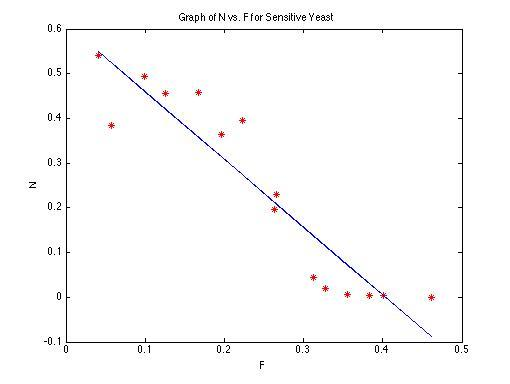
\includegraphics[width=0.5\textwidth]{images/sensitiveFit.jpg}
  \caption{\footnotesize Sensitive yeast $S$ steady-state best-fit line using Eq.\ (5).}
\end{figure}
\begin{center}
\begin{tabular}{l | c c c}
  & Estimates & SE & CI \\ 
  \hline
  $\alpha_S$ & 0.0325  & 0.0024 & (0.0255,  0.0399) \\
  $K_S$      & 20.1818 & 1.0802 & (16.9281, 23.4356) \\
\end{tabular}
\end{center}
The results on the left show that there may be a better fit to the data than Eq.\ (5).  Notice that elimination of the last few data points corresponding to high $F$ may be removed; this would reduce the standard error and hence provide a better estimate for $\alpha_L$ and $K_L$.
\end{multicols}

\begin{multicols}{2}
\begin{figure}[H]
  \centering
    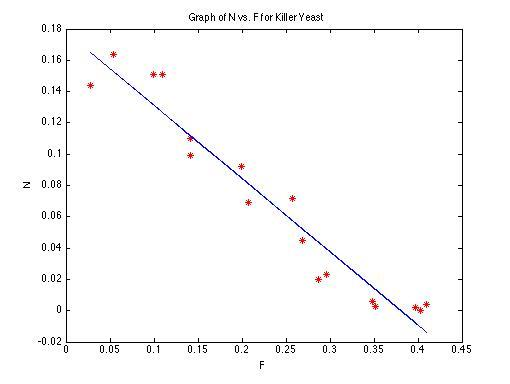
\includegraphics[width=0.5\textwidth]{images/killerFit.jpg}
  \caption{\footnotesize Killer yeast $L$ steady-state best-fit line using Eq.\ (5).}
\end{figure}
\begin{center}
\begin{tabular}{l | c c c}
  & Estimates & SE & CI \\ 
  \hline
  $\alpha_L$ & 0.1124  & 0.0053 & (0.0969,  0.1279) \\
  $K_L$      & 19.0288 & 0.6367 & (17.1526, 20.905) \\
\end{tabular}
\end{center}
The best-fit line on the left shows that steady-state data follows a fairly linear relationship with flow, and as such we can be confident our estimates for $\alpha_L$ and $K_L$ are correct.
\end{multicols}

Now that we have estimates for all values of $\alpha$ and $K$ (for both killer and sensitive yeast) we can run the dynamic model (6), (7), and (8) to equilibrium.  By letting $\beta$ range from 0 to 0.5 (in units 1/time), and $F$ range from 0 to 0.5 (in units volume/time), we can run the model for each $\beta$ and $F$ to determine the regions in the $\beta$, $F$ plane where sensitive yeast $S$ overtakes the killer yeast $L$ and vice versa.
\begin{figure}[H]
  \centering
    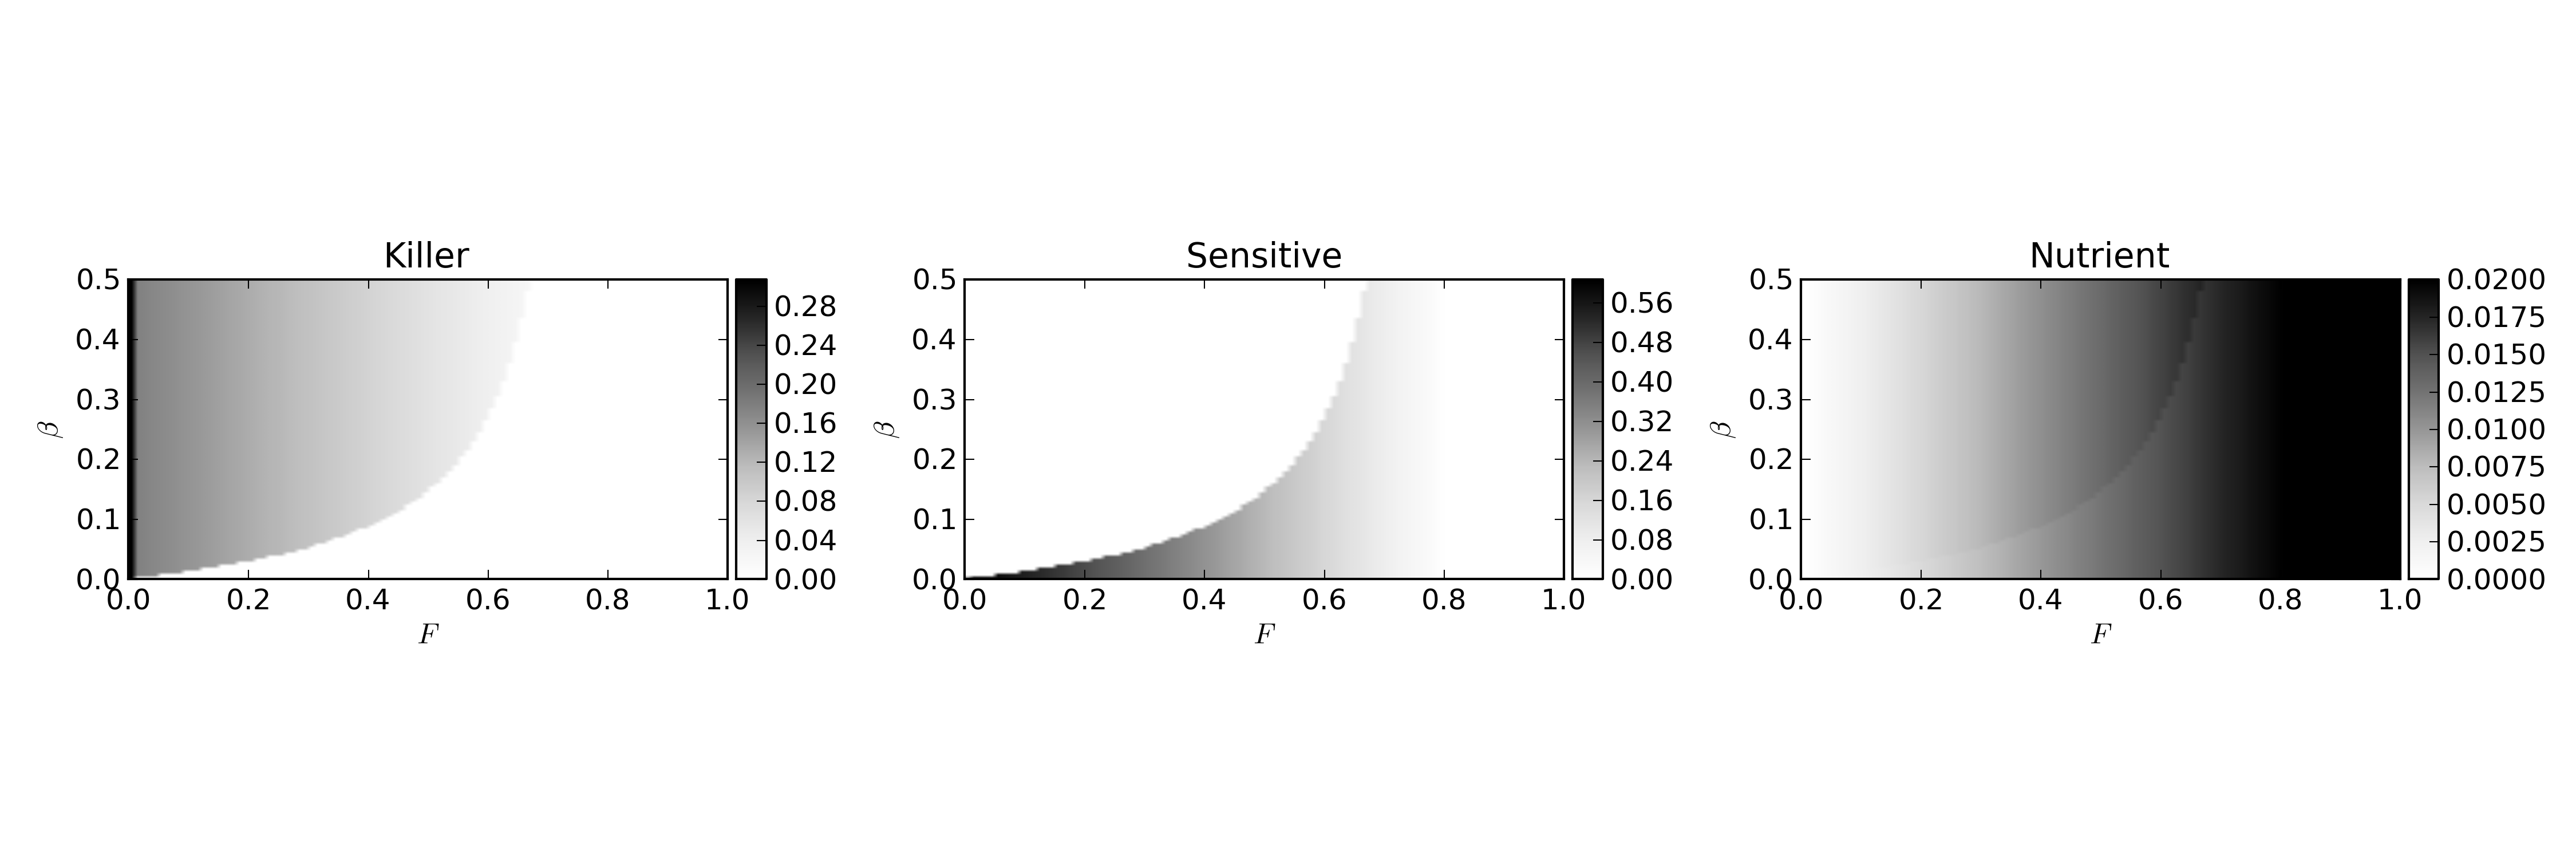
\includegraphics[width=1.0\textwidth]{images/sols.png}
  \caption{\footnotesize $250 \times 250$ steady-state optical density solution for killer yeast (left), sensitive yeast (middle) and nutrient (right) for a total run time of 40,000 hours.  Equations (6), (7), and (8) were solved with the Dormand-Prince numerical integration algorithm with an absolute tolerance of 1e-6, relative tolerance of 1e-6, and timestep $\Delta t$ of 500 hours.  The timestep was kept high due to the $250 \times 250 = 62,500$ simulations required to complete the figure.  Parallel processing was also implemented to speed up the simulation.}
\end{figure}

Notice in Figure 4 that as $\beta$ increases the killer yeast dominates and sensitive yeast eventually dies off, while as $F$ increases the sensitive yeast dominates and the killer yeast eventually dies out.  The sensitive yeast are flushed from the container at around $F = 0.4$ volumes/hr.

\begin{figure}[H]
  \centering
    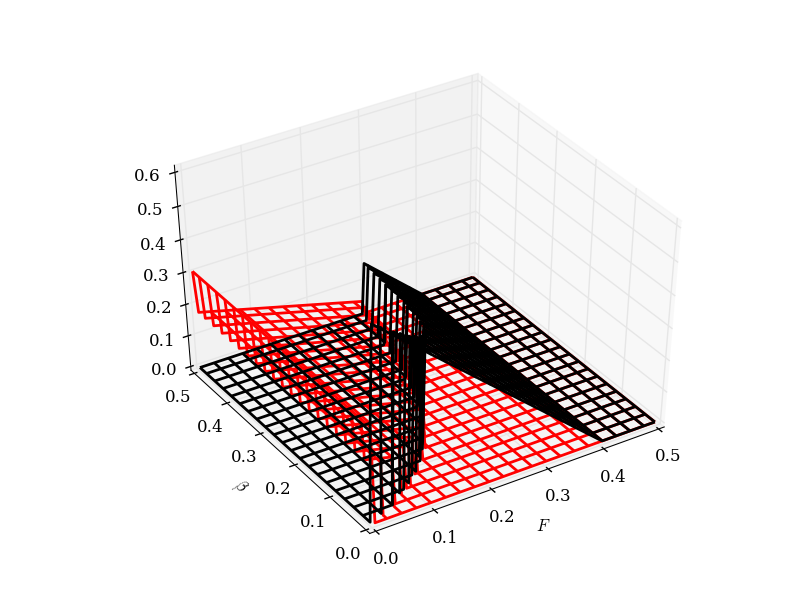
\includegraphics[width=1.0\textwidth]{images/3d.png}
  \caption{\footnotesize 3D solution depicting killer yeast (red) and sensitive yeast (black) steady-states.}
\end{figure}

\section*{Steady-State regions}

In order to evaluate the steady-state solutions, we need to equate Equations (6), (7), and (8) to zero and solve:
\begin{align}
  \frac{d}{dt}L(\bar{L}, \bar{S}, \bar{C}) &= K_L \bar{C}\bar{L} - \frac{F\bar{L}}{V} = 0, \\
  \frac{d}{dt}S(\bar{L}, \bar{S}, \bar{C}) &= K_S \bar{C}\bar{S} - \frac{F\bar{S}}{V} - \beta \bar{S} \bar{L} = 0, \\
  \frac{d}{dt}C(\bar{L}, \bar{S}, \bar{C}) &= -\alpha_L K_L \bar{C}\bar{L} -\alpha_S K_S \bar{C}\bar{S} - \frac{F\bar{C}}{V} + \frac{FC_0}{V} = 0.
\end{align}

From Eq.\ (9), we see that $\bar{L}(K_L \bar{C} - F/V) = 0$, and thus $\bar{L} = 0$ or $\bar{C} = F/(K_L V)$.  For each of these steady-states, we will evaluate Equations (10) and (11) to find the qualitative behavior of the steady-states.

\subsection*{1  $\bar{L} = 0$:}

  From (10), $\bar{S}(K_S \bar{C} - F/V - \beta \bar{L}) = 0$, so $\bar{S} = 0$ or $\bar{C} = \frac{F/V + \beta \bar{L}}{K_S} = \frac{F}{K_S V}$.
  
  \begin{enumerate}

    \item $\bar{S} = 0$:
      
    From (11), 
    \begin{align*}
      -\alpha_L K_L \bar{C}\bar{L} -\alpha_S K_S \bar{C}\bar{S} - \frac{F\bar{C}}{V} + \frac{FC_0}{V} = 0 \\
      -\frac{F\bar{C}}{V} + \frac{FC_0}{V} = 0, \hspace{5mm} F/V \neq 0.
    \end{align*}
    Thus $\bar{C} = C_0$, and the first steady-state is {\color{red}$(0,0,C_0)$}.  Call this {\color{red}Steady-State I}.

    \item $\bar{C} = \frac{F}{K_S V}$:

    From (11), 
    
    \begin{align*}
      -\alpha_S K_S \left( \frac{F}{K_S V} \right) \bar{S} - \frac{F}{V} \left( \frac{F}{K_S V} \right) + \frac{FC_0}{V} &= 0 \\
      -\alpha_S \left( \frac{F}{V} \right) \bar{S} - \frac{F}{V} \left( \frac{F}{K_S V} \right) + \frac{FC_0}{V} &= 0 \\
      \alpha_S \left( \frac{F}{V} \right) \bar{S} &= \frac{F}{V} \left( \frac{F}{K_S V} \right) - \frac{FC_0}{V} \\
      \alpha_S \bar{S} &= \frac{F}{K_S V} - C_0 \\
      \bar{S} &= \frac{F}{K_S V \alpha_S} - \frac{C_0}{\alpha_S}. \\
    \end{align*}
    Therefore, the second steady-state is {\color{red}$\left(0, \frac{F}{K_S V \alpha_S} - \frac{C_0}{\alpha_S}, \frac{F}{K_S V} \right)$}.  Call this {\color{red}Steady-State II}. 
  \end{enumerate}

\subsection*{2  $\bar{C} = \frac{F}{K_L V}$:}

  From (10), 
  \begin{align*}
    \bar{S}\left( K_S \bar{C} - \frac{F}{V} - \beta \bar{L} \right) = 0 \\
    \bar{S}\left( K_S \frac{F}{K_L V} - \frac{F}{V} - \beta \bar{L} \right) = 0.
  \end{align*}
  So $\bar{S} = 0$ or $\bar{L} = \frac{K_S F}{K_L V \beta} - \frac{F}{V \beta}$.
  
  \begin{enumerate}

    \item $\bar{S} = 0$:
      
    From (11), 
    \begin{align*}
      -\alpha_L K_L \bar{C}\bar{L} -\alpha_S K_S \bar{C}\bar{S} - \frac{F\bar{C}}{V} + \frac{FC_0}{V} &= 0 \\
      -\alpha_L \left( \frac{F}{K_L V} \right) \bar{L} - \frac{F}{V} \left( \frac{F}{K_L V} \right) + \frac{FC_0}{V} &= 0 \\
      \alpha_L \left( \frac{F}{V} \right) \bar{L} &= \frac{FC_0}{V} - \frac{F}{V} \left( \frac{F}{K_L V} \right) \\
      \alpha_L \bar{L} &= C_0 - \frac{F}{K_L V} \\
      \bar{L} &= \frac{C_0}{\alpha_L} - \frac{F}{K_L V \alpha_L}.
    \end{align*}
    Thus third steady-state is {\color{red}$\left( \frac{C_0}{\alpha_L} - \frac{F}{K_L V \alpha_L}, 0, \frac{F}{K_L V} \right)$}.  Call this {\color{red}Steady-State III}.

    \item $\bar{L} = \frac{K_S F}{K_L V \beta} - \frac{F}{V \beta}$:

    From (11), 
    \begin{align*}
      -\alpha_L K_L \bar{C}\bar{L} -\alpha_S K_S \bar{C}\bar{S} - \frac{F\bar{C}}{V} + \frac{FC_0}{V} &= 0 \\
      -\alpha_L K_L \left( \frac{F}{K_L V} \right) \left( \frac{K_S F}{K_L V \beta} - \frac{F}{V \beta} \right) -\alpha_S K_S \left( \frac{F}{K_L V} \right) \bar{S} - \frac{F}{V} \left( \frac{F}{K_L V} \right) + \frac{FC_0}{V} &= 0 
    \end{align*}
    \begin{align*}
      \implies \alpha_S K_S \left( \frac{F}{K_L V} \right) \bar{S} &=  \frac{FC_0}{V} - \alpha_L K_L \left( \frac{F}{K_L V} \right) \left( \frac{K_S F}{K_L V \beta} - \frac{F}{V \beta} \right) - \frac{F}{V} \left( \frac{F}{K_L V} \right) \\ 
      \alpha_S K_S \left( \frac{1}{K_L} \right) \bar{S} &=  C_0 - \alpha_L \left( \frac{K_S}{K_L \beta} - \frac{1}{\beta} \right) - \left( \frac{F}{K_L V} \right) \\ 
      \bar{S} &= \left( \frac{K_L}{\alpha_S K_S} \right) C_0 - \alpha_L \left( \frac{K_L}{\alpha_S K_S} \right) \left( \frac{K_S}{K_L \beta} - \frac{1}{\beta} \right) - \left( \frac{K_L}{\alpha_S K_S} \right) \left( \frac{F}{K_L V} \right) \\ 
      \bar{S} &= \frac{K_L C_0}{\alpha_S K_S} - \frac{\alpha_L}{\alpha_S \beta} + \frac{\alpha_L K_L}{\alpha_S K_S \beta} - \frac{F}{\alpha_S K_S V}.
    \end{align*}
    Therefore, the fourth and final steady-state is {\color{red}$\left(\frac{K_S F}{K_L V \beta} - \frac{F}{V \beta},\ \frac{K_L C_0}{\alpha_S K_S} - \frac{\alpha_L}{\alpha_S \beta} + \frac{\alpha_L K_L}{\alpha_S K_S \beta} - \frac{F}{\alpha_S K_S V},\ \frac{F}{K_L V} \right)$}.  Call this {\color{red}Steady-State IV}. 
  \end{enumerate}

\section*{Source Code:}

\pythonexternal{/home/pf4d/Documents/ode_plot/example/killerYeast.py}

\end{document}


